% !TeX root = ../../main.tex

For a finite point set $P\subset D$ recall that the \v Cech complex $\cech^\e(P)$ is defined to be the Nerve of the open cover $\{\ball_D^\e(p)\}_{p\in P}$.
When $\varrho_D > \e$ this cover is good, and the Nerve Theorem states that $\cech^\e(P)$ is homotopy equivalent to $P^\e$.
That is, for all $z\in\R$, $\e < \varrho_D$ we have an isomorphism $\N_z^{\e, k} : \hom_k(\cech^\e(P,Q_z))\to \hom_k(P^\e, Q_z^\e)$ on homology groups that is induced by this homotopy equivalence.

\paragraph{Duality}

The statement of Theorem~\ref{thm:geo_tcc} in terms of the $0$-dimensional homology of complement spaces makes it difficult, if not impossible, to compute directly.
% The following lemma
% Lemma~\ref{lem:duality_apply} of Appendix~\ref{apx:duality} applies Alexander Duality (see Lemma~\ref{cor:alexander_iso}) and the Universal Coefficient Theorem to equate the $d$-dimensional homology of cover to $0$-dimensional homology of their complements.
For finitely generated (co)homology over a field the Universal Coefficient Theorem can be used with Alexander Duality to show $\hom_d(P^\e,Q_z^\e)\cong\hom_0(D\setminus Q_z^\e, D\setminus P^\e)$.
 % give a natural isomorphism $\xi_z^\e : \hom_d(P^\e,Q_z^\e)\to \hom_0(D\setminus Q_z^\e, D\setminus P^\e)$.\footnote{For the construction of this isomorphism see the \fullversion.}
This isomorphism holds in the specific case when $P^\e\subseteq \intr_\X(D)$ and $D\setminus P^\e$, $D\setminus Q_z^\e$ are locally contractible.
We therefore provide the following definition for ease of exposition.
\begin{definition}[$(\omega, \delta,\zeta)$-Sample]
  For $\zeta\geq \delta > 0$, $\omega\in\R$, and a $c$-Lipschitz function $f: D\to \R$ a finite point set $P\subset D$ is said to be an \textbf{$(\omega, \delta, \zeta)$-sample} of $f$ if \begin{itemize}
    \item $P^\delta\subset\intr_\X(D)$ and
    \item $D\setminus P^\delta$, $D\setminus Q_{\omega-c\zeta}^\delta$, and $D\setminus Q_{\omega+c\delta}^\delta$ are locally path connected in $\X$.
  \end{itemize}
\end{definition}

The requirement that our complements are locally path connected is necessary in order to satisfy the general statement of the duality theorem.
A rigorous investigation of the minimal assumptions that can be made on $\X$ and $D$ is beyond the scope of this paper.
We note that, in practice, it likely suffices to assume that there exists a triangulation of $P^\e$ that is a subcomplex of some refinement of a triangulation of $\X$ (see~\cite{cavanna2017when},~\cite{julian83alexander}).

\paragraph{Assumption 2}

In order obtain an upper bound on $\rk~j$ we introduce our second assumption: that $\hom_0(D\setminus B_\omega\hookrightarrow D\setminus B_{\omega-c(\delta+\zeta)})$ is \emph{injective}---as we move away from $\omega$ moving \emph{down} no components \emph{disappear}.
Once again, in terms of $\omega$ as a superlevel set monotonically decreasing, no components \emph{disappear} right \emph{after} $\omega$.
For a function in two dimensions, this translates to features in dimension 1 appearing before $\omega$ in the sublevel set filtration, as shown in Figure~\ref{fig:assumption2}.
% Once again, in terms of $\omega$ as a sub-levelset monotonically increasing, no components \emph{appear} right \emph{before} $\omega$.

% \begin{figure}[htbp]\label{fig:assumption_2}
%   \centering
%   % 
\includegraphics[trim=50 190 0 200, clip, scale=0.2]{scripts/figures/scalar.png}
%   % 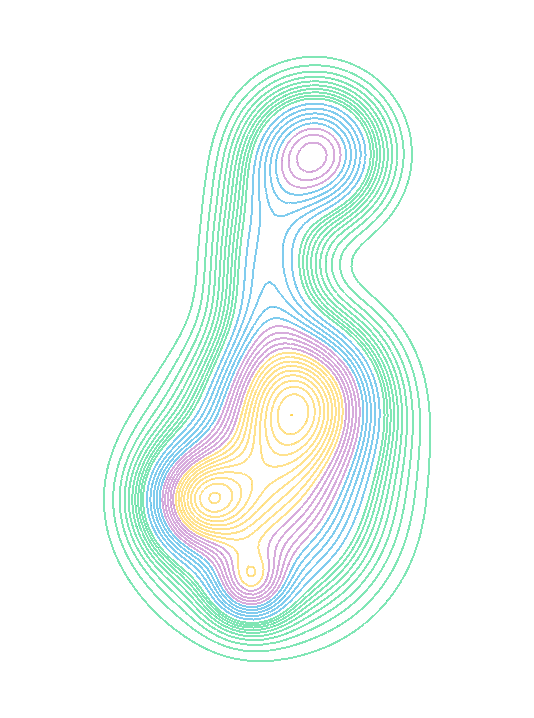
\includegraphics[trim=100 25 75 0, clip, angle=280, scale=0.25]{scripts/figures/scalar_contour.png}
%   
\includegraphics[trim=200 325 150 300, clip, scale=0.3]{scripts/figures/scalar_a2_B.png}
%   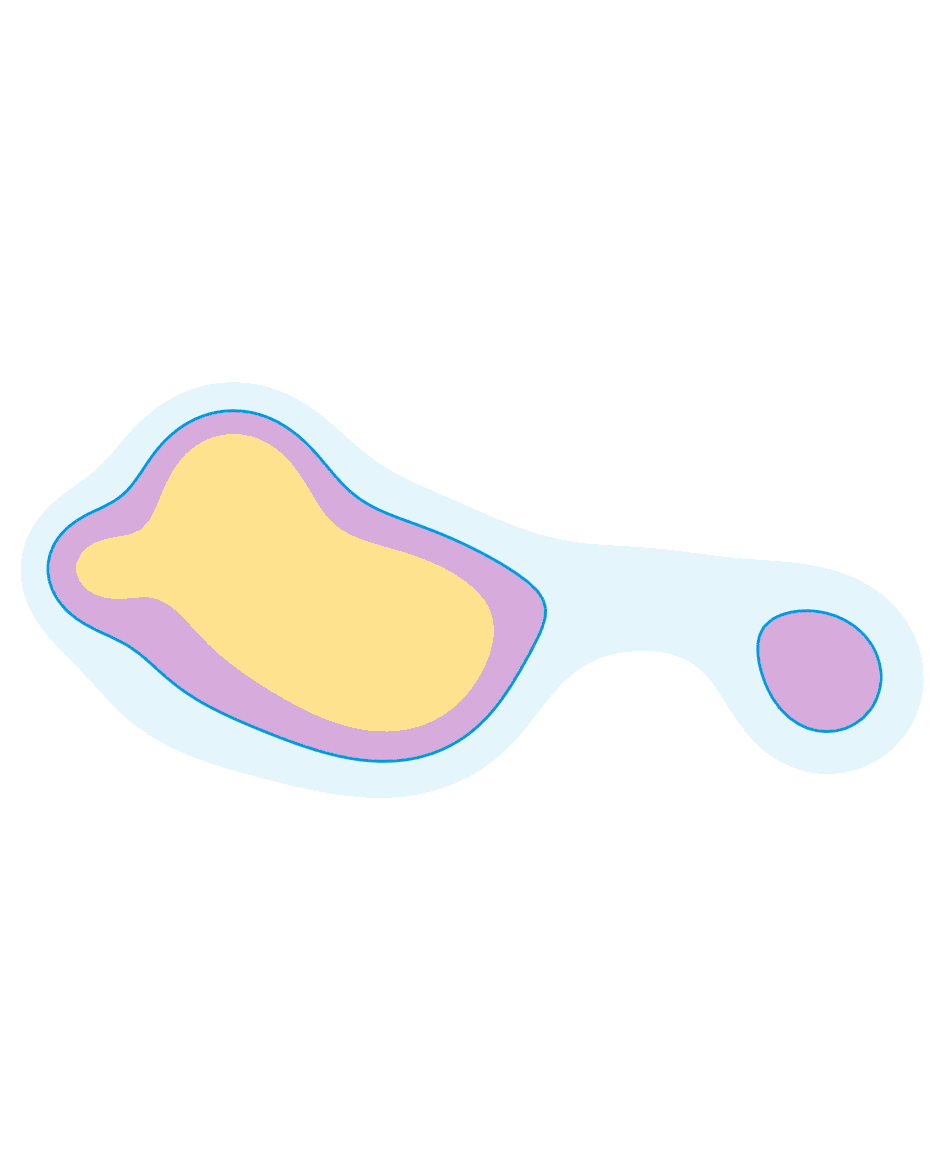
\includegraphics[trim=0 350 0 370, clip, scale=0.2]{scripts/figures/scalar_a2_B_top.png}
%   
\includegraphics[trim=200 325 150 300, clip, scale=0.3]{scripts/figures/scalar_a2_A.png}
%   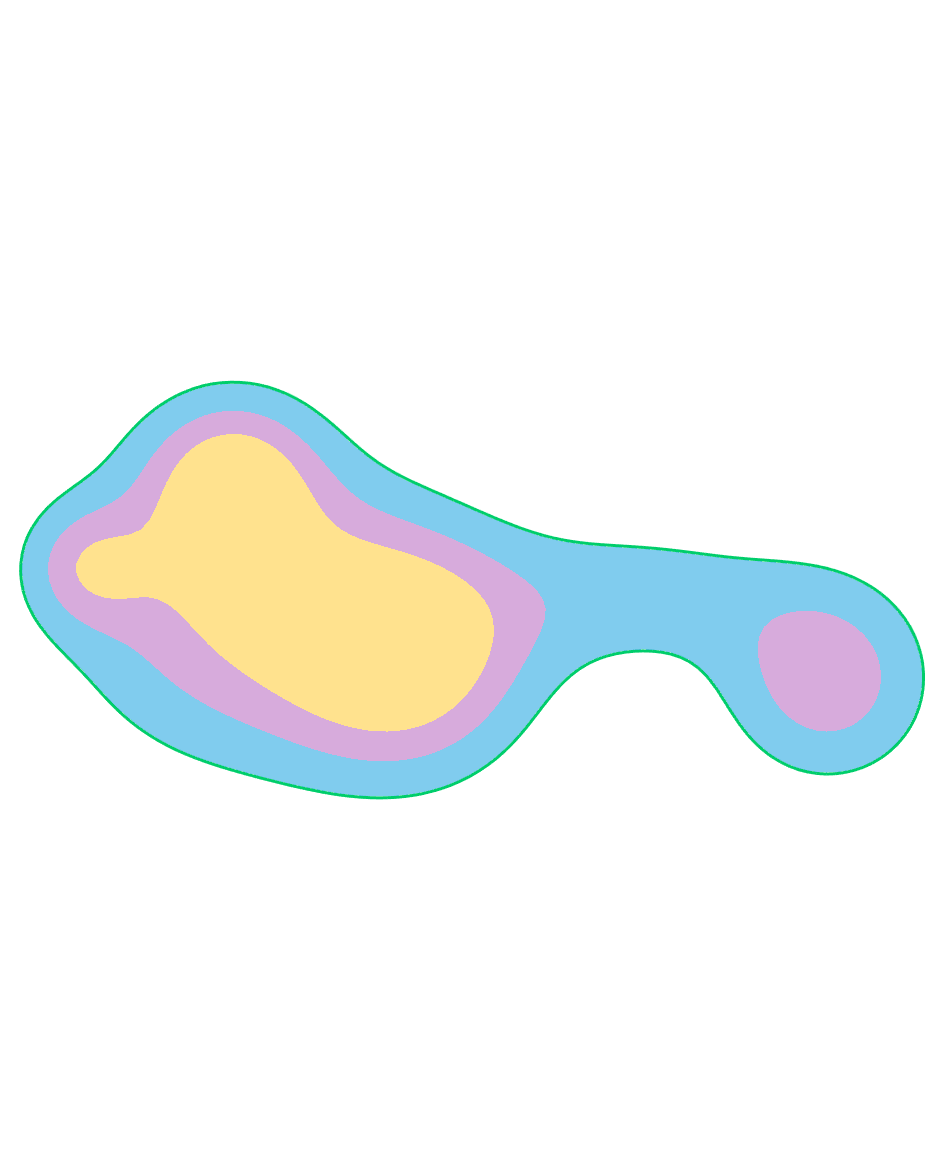
\includegraphics[trim=0 350 0 370, clip, scale=0.2]{scripts/figures/scalar_a2_A_top.png}
%   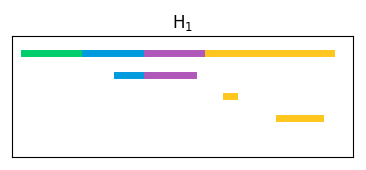
\includegraphics[scale=0.7]{scripts/figures/scalar_barcode_H1.png}
%   % \includegraphics[scale=0.55]{scripts/figures/scalar_barcode_super_0.png}
%   % \includegraphics[scale=0.55]{scripts/figures/scalar_barcode_sub_1.png}
%   \caption{\textbf{(Assumption 2)} The blue levelset does not satisfy Assumption 2 as the smaller component is not in the inclusion from blue to green.
%           This can be seen in the second feature of the barcode shown as a feature which is born in the blue region.}
% \end{figure}

\begin{figure}[htbp]\label{fig:assumption2}
  \centering
  % 
\includegraphics[trim=50 190 0 200, clip, scale=0.2]{scripts/figures/scalar.png}
  % 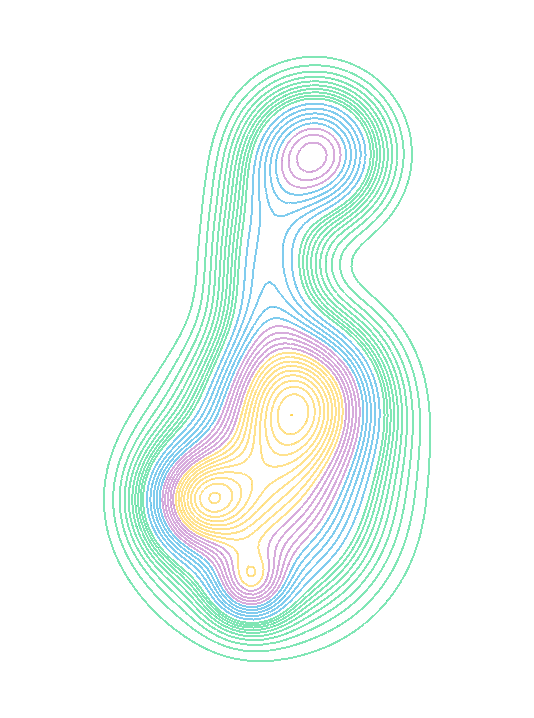
\includegraphics[trim=100 25 75 0, clip, angle=280, scale=0.25]{scripts/figures/scalar_contour.png}
  
\includegraphics[trim=200 300 200 200, clip, width=0.5\textwidth]{figures/surf-ass2_C_side.png}
  
\includegraphics[trim=300 200 200 200, clip, width=0.3\textwidth]{figures/surf-ass2_C_top.png}
  
\includegraphics[trim=200 300 200 200, clip, width=0.5\textwidth]{figures/surf-ass2_B_side.png}
  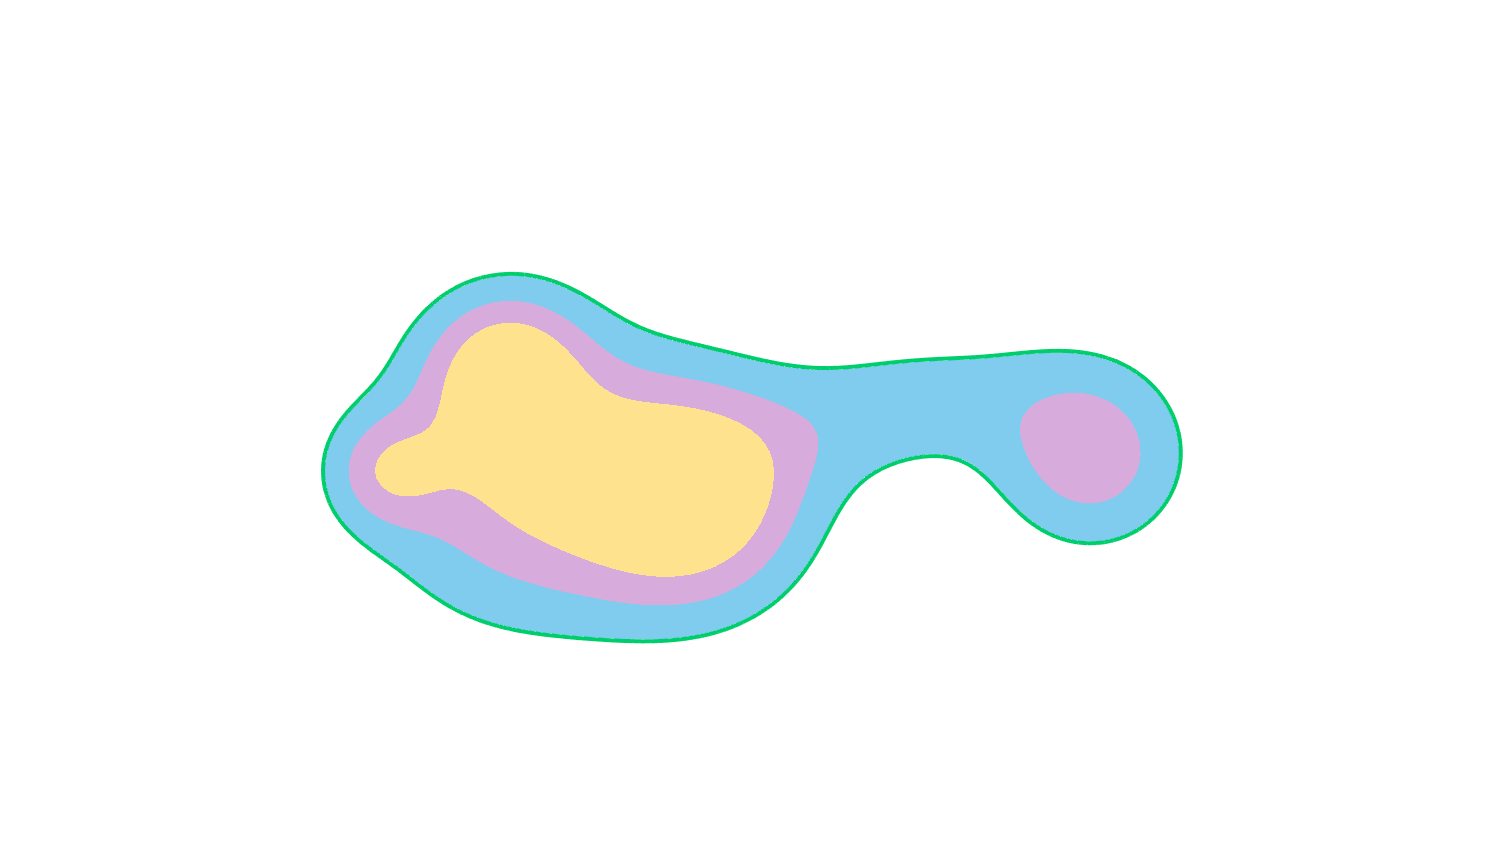
\includegraphics[trim=300 200 200 200, clip, width=0.3\textwidth]{figures/surf-ass2_B_top.png}
  
\includegraphics[scale=0.7]{figures/scalar_barcode_H1-masked.png}
  \caption{\textbf{(Assumption 2)} The blue levelset does not satisfy Assumption 2 as the smaller component is not in the inclusion from blue to green.
          This can be seen in the second feature of the barcode shown that is born in the blue region.}
\end{figure}

\begin{lemma}\label{lem:assumption2}
  If $\hom_0(D\setminus B_\omega\hookrightarrow D\setminus B_{\omega+c(\delta+\zeta)})$ is injective and each component of $D\setminus B_\omega$ contains a point in $P$ then $\dim~\hom_0(\rips^\delta(P\setminus Q_{\omega-c\zeta})) \geq \dim~\hom_0(D\setminus B_\omega)$.
\end{lemma}
\begin{proof}
  Assume there exist $p,q \in P\setminus Q_{\omega-c\zeta}$ such that $p$ and $q$ are connected in $\rips^\delta(P\setminus Q_{\omega-c\zeta})$ but not in $D\setminus B_\omega$.
  So the shortest path from $p, q$ is a subset of $(P\setminus Q_{\omega-c\zeta})^\delta$.
  For any $x\in (P\setminus Q_{\omega-c\zeta})^\delta$ there exists some $p\in P$ such that $f(p) > \omega - c\zeta$ and $\dist(p,x) < \delta$.
  Because $f$ is $c$-Lipschitz
  \[ f(x)\geq f(p) - c\dist(x,p) > \omega - c(\delta+\zeta)\]
  so there is a path from $p$ to $q$ in $D\setminus B_{\omega-c(\delta+\zeta)}$, thus $[p] = [q]$ in $\hom_0(D\setminus B_{\omega-c(\delta+\zeta)})$.

  But we have assumed that $[p]\neq[q]$ in $\hom_0(D\setminus B_\omega)$, contradicting our assumption that $\hom_0(D\setminus B_\omega\hookrightarrow D\setminus B_{\omega-c(\delta+\zeta)})$ is injective, so any $p,q$ connected in $\rips^\delta(P\setminus Q_{\omega-c\zeta})$ are connected in $D\setminus B_\omega$.
  That is, $\dim~\hom_0(\rips^\delta(P\setminus Q_{\omega-c\zeta}))\geq \dim~\hom_0(D\setminus B_\omega)$.
\end{proof}

\paragraph{Rips Approximation}

We would now like to compute the TCC by factoring an inclusion of Rips complexes through that of the \v Cech.
This will give us a lower bound on the rank of the map induced on $d$-dimensional homology which can then be used to confirm coverage via Lemma~\ref{lem:duality_apply}.
We have the following sequence of homomorphisms induced by inclusions
\[ \hom_k(\rips^\e(P, Q_w))\xrightarrow{J_w^\e}\hom_k(\cech^\e(P, Q_w))\xrightarrow{I_w^\e}\hom_k(\rips^\e(P, Q_w))\]
so that, for any $w\leq z$, $\e\leq\eta < \varrho_D$ and $q_{\rips} : \hom_k(\rips^\e(P, Q_w))\to \hom_k(\rips^{2\eta}(P, Q_z))$, $q_{\cech} : \hom_k(\cech^\e(P, Q_w))\to \hom_k(\cech^{\eta}(P, Q_z))$ induced by inclusions, $q_{\rips}$ factors through $q_{\cech}$ as $q_{\rips} = I_z^\eta\circ q_{\cech}\circ J_w^\e$.

% Lemma~\ref{lem:pers_nerve_filt} (see Appendix~\ref{apx:nerves}) adapts the persistent nerve lemma of Chazal et. al.~\cite{chazal08towards} (see Appendix~\ref{apx:nerves}, Lemma~\ref{lem:pers_nerve}) to the relative case.
% That is, to show the isomorphisms $\N_w^\e$ and $\N_z^\eta$ commute with maps $q_{\cech}$ and $q : \hom_k(P^\e, Q_w^\e)\to\hom_k(P^\eta, Q_z^\eta)$  induced by inclusion.%, thus $\rk~q = \rk~q_{\cech} \geq \rk~q_{\rips}$.

\begin{theorem}[Algorithmic TCC]\label{thm:algo_tcc}
  Let $\X$ be an orientable $d$-manifold and let $D$ be a compact subset of $\X$.
  Let $f : D\to\R$ be a $c$-Lipschitz function and $\omega\in\R$, $\delta\leq\zeta < \varrho_D$ be constants such that $B_{\omega - c(\zeta +\delta)}$ surrounds $D$ in $\X$.
  Let $P$ be an $(\omega, \delta,\zeta)$-sample of $f$ such that every component of $D\setminus B_\omega$ contains a point in $P$.
  Suppose $\hom_0(D\setminus B_{\omega+c(\delta+\zeta)}\hookrightarrow D\setminus B_\omega)$ is surjective and $\hom_0(D\setminus B_\omega\hookrightarrow D\setminus B_{\omega-c(\delta+\zeta)})$ is injective.

   If $\rk~\hom_d(\rips^\delta(P, Q_{\omega -c\zeta})\hookrightarrow \rips^{2\delta}(P, Q_{\omega+c\delta})) \geq \dim~\hom_0(\rips^\delta(P\setminus Q_{\omega-c\zeta}))$ then $D\setminus B_\omega\subseteq P^\delta$ and $Q_{\omega-c\zeta}^\delta$ surrounds $P^\delta$ in $D$.
\end{theorem}
\begin{proof}
  Let $q : \hom_d(P^\delta, Q_{\omega-c\zeta}^\delta)\to \hom_d(P^\delta, Q_{\omega+c\delta}^\delta)$,
  $q_{\cech} : \hom_d(\cech^{\delta}(P, Q_{\omega-c\zeta}))\to\hom_d(\cech^{\delta}(P, Q_{\omega+c\delta}))$, and
  $q_{\rips} : \hom_d(\rips^{\delta}(P, Q_{\omega-c\zeta}))\to\hom_d(\rips^{2\delta}(P, Q_{\omega+c\delta}))$ be induced by inclusion.
  Then $\rk~q_{\cech} \geq\rk~q_{\rips}$ as $q_{\rips}$ factors through $q_{\cech}$ by the Rips-\v Cech interleaving.
  Moreover, $\rk~q = \rk~q_{\cech}$ by the Persistent Nerve Lemma, so $\rk~q\geq \rk~q_{\rips}$.
  As we have assumed $\hom_0(D\setminus B_\omega\hookrightarrow D\setminus B_{\omega-c(\delta+\zeta)})$ is injective Lemma~\ref{lem:assumption2} implies $\dim~\hom_0(\rips^\delta(P\setminus Q_{\omega-c\zeta}))\geq \dim~\hom_0(D\setminus B_\omega)$.
  Because $P$ is an $(\omega, \delta, \zeta)$-sample of $f$ we have $\hom_d(P^\delta, Q_{\omega-c\zeta}^\delta)\cong \hom_0(D\setminus Q_{\omega-c\zeta}^\delta, D\setminus P^\delta)$ and $\hom_d(P^\delta, Q_{\omega+c\delta}^\delta)\cong \hom_0(D\setminus Q_{\omega+c\delta}^\delta, D\setminus P^\delta)$ so $\rk~i\geq \rk~q$ by Alexander Duality and the Universal Coefficient Theorem.
  So, by our hypothesis that $\rk~q_{\rips}\geq\dim~\hom_0(\rips^\delta(P\setminus Q_{\omega-c\zeta}))$ we have $\rk~i\geq\dim~\hom_0(D\setminus B_\omega)$.

  As $j : \hom_0(D\setminus B_{\omega+c(\delta+\zeta)})\to \hom_0(D\setminus B_\omega)$ is surjective by assumption $\rk~j = \dim~\hom_0(D\setminus B_\omega)$, so $D\setminus B_\omega\subseteq P^\delta$ and $Q_{\omega-c\zeta}^\delta$ surrounds $P^\delta$ in $D$ by Theorem~\ref{thm:geo_tcc} as desired.
\end{proof}
